\documentclass{VUMIFInfKursinis}
\usepackage{algorithmicx}
\usepackage{algorithm}
\usepackage{algpseudocode}
\usepackage{amsfonts}
\usepackage{amsmath}
\usepackage{bm}
\usepackage{color}
\usepackage{graphicx}
% \usepackage{hyperref}  % Nuorodų aktyvavimas
\usepackage{url}
\usepackage{csquotes}
\usepackage{subcaption}

% spalvos:
\usepackage{xcolor}
\definecolor{raudona}{RGB}{202,82,61}
\definecolor{zalia}{RGB}{133,181,98}
\definecolor{melyna}{RGB}{46,75,167}




% Titulinio aprašas
\university{Vilniaus universitetas}
\faculty{Matematikos ir informatikos fakultetas}
\department{PROGRAMŲ SISTEMŲ BAKALAURO STUDIJŲ PROGRAMA}
\papertype{Kursinis darbas}
\title{Dirbtinio intelekto modelių kolapsas}
\titleineng{Artificial intelligence model collapse}
\status{4 kurso 1 grupės studentė}
\author{Greta Virpšaitė}
\supervisor{j. asist. Boleslovas Dapkūnas}
\date{Vilnius \\ \the\year}


\bibliography{bibliografija} 

\begin{document}
\maketitle

\tableofcontents

\sectionnonum{Įvadas}
% Įvade apibūdinamas darbo tikslas, temos aktualumas ir siekiami rezultatai.
Dirbtinio intelekto (DI) kūrimas ir pritaikymas šiandien yra svarbesnis nei bet kada anksčiau. Ši technologija pritaikoma praktiškai kiekvienoje pramonės šakoje, o kai kuriose srityse, pavyzdžiui, gyvybės gelbėjimo technologijose, DI tampa nepakeičiamas. Medicinoje DI padeda įtarti odos vėžį, (pvz. melanomą \cite{Melanoma}), ekstremalių situacijų valdymo srityje prognozuoti žemės drebėjimus \cite{Drebejimai} ar cunamius \cite{Cunamiai}, o tai gelbsti gyvybes. Todėl tampa būtina užtikrinti, kad DI modelius naudojančios sistemos generuodamos informaciją ją pateiktų korektiškai.

Tobulėjant DI technologijoms, vis labiau išryškėja tokios problemos kaip DI modelių kolapsas (angl. \textsl{AI model collapse}). Šis reiškinys šaltinyje \cite{AICollapseNature} apibūdinamas kaip procesas, kurio metu DI modeliai (šiuo atveju generatyvinis intelektas (GenAI)), iteratyviai mokydamiesi naudodami jų pačių sugeneruotus duomenimis, praranda gebėjimą tiksliai atspindėti pradinę duomenų informaciją. Terminas \enquote{DI modeliai} \cite{AICollapseNature} straipsnyje ir kituose šios temos darbuose (\cite{DesniuPasiulymai, modelCollapseRef}, naudojamas kaip sinonimas giliųjų neuroninių tinklų apibūdinimui, nes tyrimuose nagrinėjami tik jie. Ši problema ypač aktuali, žinant kaip plačiai yra naudojami kompanijos \enquote{OpenAI} DI produktai kaip \enquote{DALL-E},\enquote{GPT}, \enquote{Sora}, o jų sugeneruoti rezultatai internete gali užteršti būsimus mokymosi duomenų rinkinius. Šių produktų naudojimas pamažu plinta į visas industrijas, todėl DI modelių kolapsas gali lemti nekorektiškos informacijos skleidimą, kuris potencialiai pakenktų vartotojams.  

Pastarųjų metų tyrimai nustatė keletą mechanizmų ir rizikų, susijusių su DI modelių kolapsu. Pavyzdžiui, tyrime 
\cite{ModelsGoMAD} apibrėžiama, kaip rekursiniai mokymo ciklai (angl. \textsl{recursive training loops}), tokie kaip visiškai sintetiniai ciklai (angl. \textsl{fully synthetic loops}), sintetiniai augmentacijų ciklai (angl. \textsl{synthetic augmentation loops}) ir ciklai su šviežiais duomenimis (angl. \textsl{fresh data loops}), gali skirtingai paspartinti modelių kolapsą. 

% Kitas tyrimas \cite{FairnessFeedbackLoops} akcentuoja, kaip grįžtamojo ryšio ciklai (angl. \textsl{feedback loops}) gali sustiprinti DI modelių etinį šališkumą (angl. \textsl{bias amplification})}. 

Shumailov et al. tyrime \cite{AICollapseNature} pateikia pagrindines kolapso apibrėžtis bei su kolapsu susijusias klaidas, kurios padeda giliau suprasti, kaip galima atpažinti DI modelių kolapsą.

Svarbu paminėti, kad Europos Sąjungos pasiūlytas Dirbtinio intelekto aktas \cite{AIEuropeanAct} gali svariai prisidėti prie DI modelių kolapso problematikos sprendimo. Jame pateikti reglamentai netiesiogiai gali prisidėti prie kai kurių DI sistemų kolapso rizikos mažinimo. Toks taikymas yra itin svarbus didelės rizikos DI sistemoms.


% Šis darbas giliau aptars DI kolapso mechanizmus, atpažinimo technikas, galimas prevencines priemones ir paaiškins, kaip įvyksta kolapsas. Taip pat, darbe bus pateiktos įžvalgos apie tai, kokį poveikį modelių kolapsas galėtų turėti, jei nesiimama tinkamų reguliavimo veiksmų.


\textbf{Darbo tikslas} – giliau išnagrinėti DI modelių kolapso mechanizmus,  šiuolaikinius mokslinius metodus, skirtus šios problemos identifikavimui ir sprendimui, su tikslu pateikti įžvalgas apie galimas prevencines priemones ir jų implementavimą kasdienėje praktikoje.

\textbf{Uždaviniai:}
\begin{enumerate}
    \item Išanalizuoti literatūrą, susijusią su DI modelių kolapsu, apimant pagrindinius mechanizmus, rizikas ir galimus sprendimus. Aprašyti DI modelių kolapso atpažinimo technikas, remiantis šiuolaikiniais tyrimais.
    \item Apibrėžti pagrindines DI modelių kolapso prevencijos strategijas, įtraukiant Europos Sąjungos DI aktą ir jo įtaką DI modelių stabilumui.
    \item Atlikti eksperimentą su VAE modeliu, mokant jį MNIST duomenų rinkiniu, siekiant ištirti modelio kolapso reiškinį.
    \item Aptarti etines implikacijas, susijusias su DI modelių kolapsu ir jo prevencija.
    \item Parengti rekomendacijas, pagrįstas atliktos analizės rezultatais, kurios galėtų būti pritaikomos moksliniuose ir praktiniuose kontekstuose.
\end{enumerate}





\section{DI modelių kolapsas}
% Pagrindinėje tiriamojoje dalyje aptariama ir pagrindžiama tyrimo metodika;
% pagal atitinkamas darbo dalis, nuosekliai, panaudojant lyginamosios analizės,
% klasifikacijos, sisteminimo metodus bei apibendrinimus, dėstoma sukaupta ir
% išanalizuota medžiaga.

% Šioje dalyje aptariama skirtingą literatūra DI modelių kolapso tematika. 

\subsection{Kas yra DI modelių kolapsas?}
Šio termino apibrėžimas yra gana naujas, tačiau dažniausiai DI modelių kolapso tema remiamasi \enquote{Nature} žurnale publikuotu straipsniu \cite{AICollapseNature}.

Shumailov et al. tyrime \cite{AICollapseNature} pateikia pagrindinį DI modelių kolapso apribrėžimą kaip kaip degeneratyvų procesą, kuris atsiranda, kai generatyviniai modeliai mokomi naudojant jų pačių sugeneruotus duomenis. Autoriai teigia, jog tai lemia vis didesnį mokymo duomenų užterštumą ir, galiausiai, modeliai pradeda klaidingai suvokti tikrovę.

Autoriai tame pačiame straipsnyje taip pat paryškina, kad yra dviejų tipų DI modelių kolapsas: ankstyvasis DI modelių kolapsas (angl. \textsl{early AI model collapse}) ir vėlyvasis DI modelių kolapsas (angl. \textsl{late AI model collapse}). Ankstyvasis DI modelių kolapsas, tai, kai modelis pradeda prarasti informaciją apie skirstinio kraštus (angl. \textsl{tails of a distribution}). Tai reiškia, kad rečiau naudojami duomenų elementai gali išnykti ankstyvuosiuose mokymo etapuose. Skirstinio kraštų paaiškinimas žr. \ref{img:uodegos} pav. 


\begin{figure}[H]
    \centering
    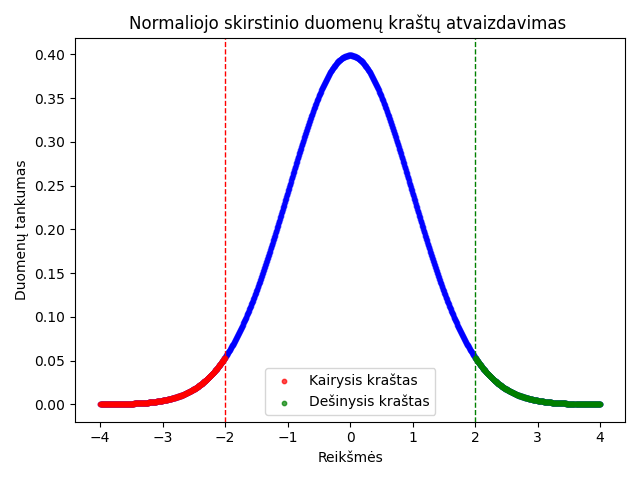
\includegraphics[scale=0.6]{img/normaliojo_skirstinio_grafikas.png}
    \caption{\textbf{Teorinis normaliojo skirstinio duomenų kraštų atvaizdavimas pagal \cite{Statistika} knygoje pateikiamą informaciją}. Tai toks skirstinys, kai duomenys yra simetriškai pasiskirstę aplink vidurį, o retesni duomenys yra kraštuose. \textcolor{raudona}{Kairysis kraštas (raudona)} vaizduoja mažo tankio, retai pasitaikančius duomenis vienoje skirstinio pusėje, o \textcolor{zalia}{dešinysis kraštas (žalia)} rodo panašaus pobūdžio retus duomenis kitoje pusėje.}  
    \label{img:uodegos}
\end{figure}


Vėlyvasis modelių kolapsas įvyksta tada, kai modelis konverguoja į skirstinį, kuris beveik visiškai neatitinka pradinio. Pavyzdžiui, pradinis skirstinys gali būti normalusis skirstinys, tačiau po modelio kolapso jis pasikeičia į visiškai kitokį, kuris nebeatspindi pradinės duomenų struktūros .


Verta paminėti, kad DI modelių kolapsą galima aiškiai pastebėti vizualiai analizuojant jų išvestis. Pavyzdžiui, straipsnyje \cite{AICollapseNature} pateikiamas kelių generacijų modelio degradavimo procesas anglų kalba. (žr. \ref{img:textCollapse} pav.)

\begin{figure}[H]
    \centering
    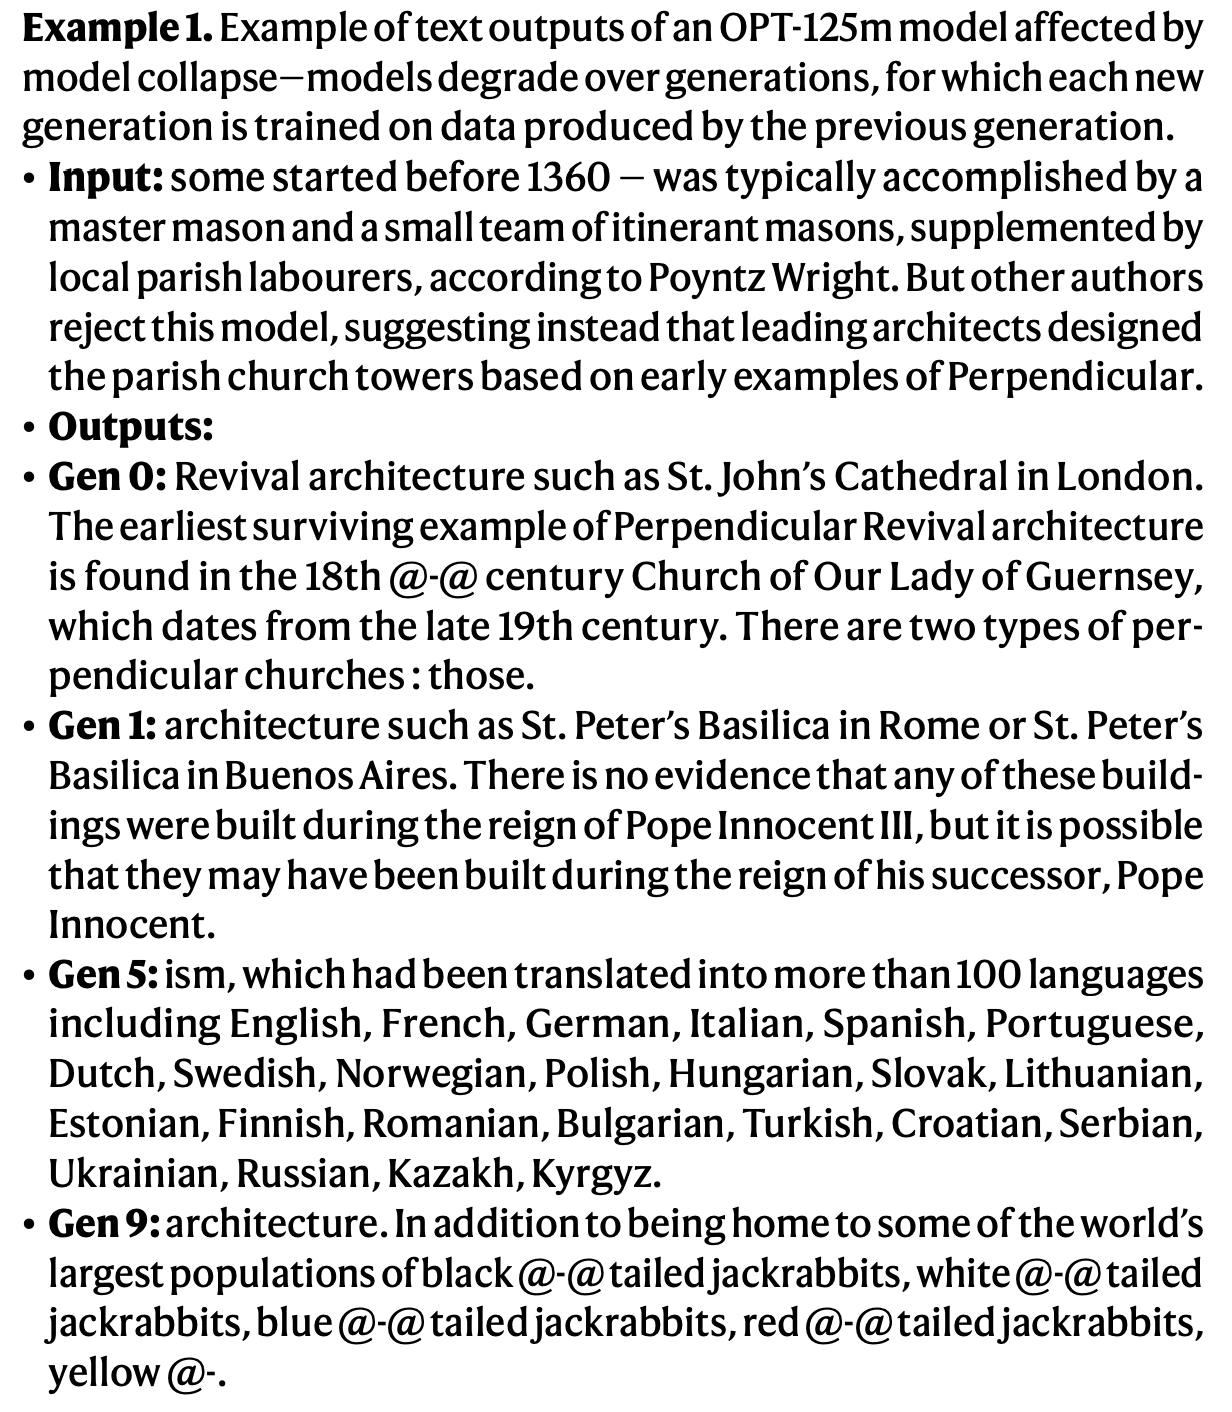
\includegraphics[scale=0.5]{img/natureTextCollapse.png}
    \caption{\textbf{Modelio OPT-125m DI kolapso pavizdys iš \cite{AICollapseNature}}. Paveiksle esančiame tekste matoma, jog generacijų skaičiui didėjant (angl. \textsl{generation} (Gen.)) didėja pasikartojančių frazių skaičius išvestyse (\enquote{gen 9} ypač dažnai kartojasi frazė \enquote{ tailed jackrabbits}. Teksto logika taip pat pasikeičia. Pirminė įvestis kalba apie architektūrą, o \enquote{gen 9} kalbama apie triušių tipus.}  
    \label{img:textCollapse}
\end{figure}


Ankstyvosiose generacijose modelio išvestys dar išlaiko sakinių logiką, galima suprasti pagrindinę teksto mintį, o frazės nėra dažnai kartojamos. Tačiau vėlesnėse generacijose pastebima, kad žodžiai pradeda kartotis vis dažniau, tekstas praranda loginę struktūrą, o sakiniai tampa visiškai nelogiški.

Panašus procesas pastebimas ir nuotraukas generuojančiuose DI modeliuose, kaip aprašyta straipsnyje \cite{ModelsGoMAD} (žr. \ref{img:nuotraukuKolapsas} pav.). Čia matoma, kad didėjant generacijų skaičiui modelis pradeda kurti vis panašesnes žmonių nuotraukas. Vėlesnėse generacijose beveik visi žmonės yra vienodos odos spalvos, jų veiduose matoma vienoda šypsena, o nuotraukų fonai tampa vienodi – dažniausiai žali arba pilki. 

\begin{figure}[H]
    \centering
    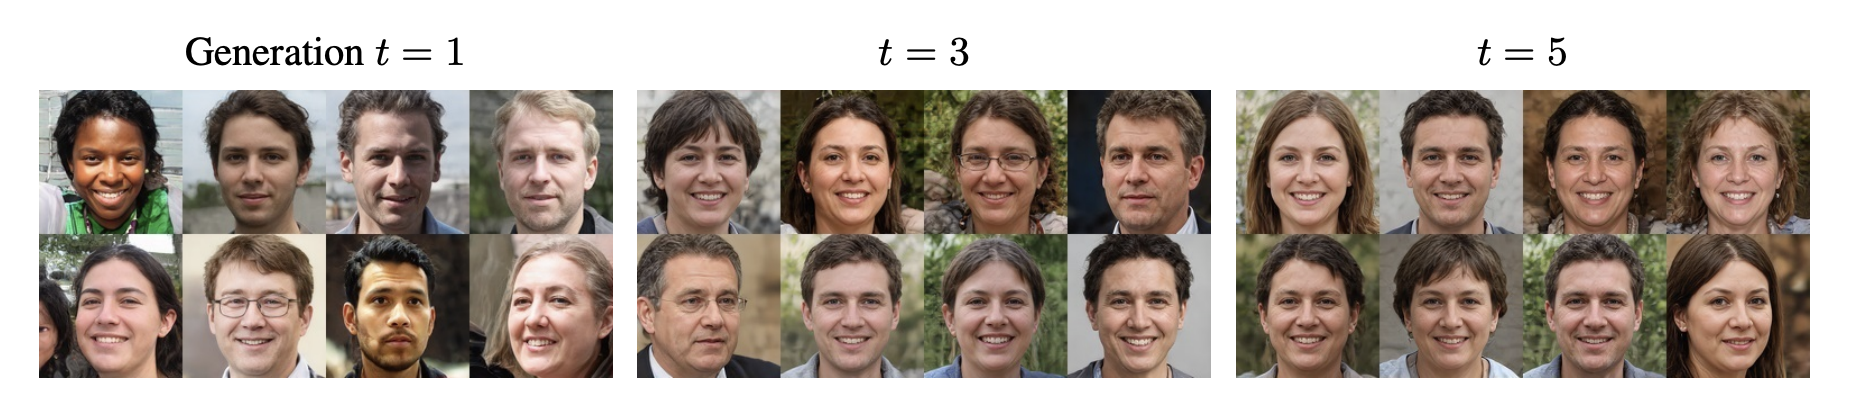
\includegraphics[scale=0.5]{img/nuotraukuKolapsas.png}
    \caption{\textbf{\cite{ModelsGoMAD} straipsnyje pateiktas skirtingų modelio iteracijų generuojamų nuotraukų pavyzdys.}. Nuotraukose matoma, kaip keičiantis t (generacijų (angl. \textsl{generations}) skaičiui) modelio įvairovė nyksta. Tai atsispindi žmonių odos ir plaukų spalvų, emocijų, drabužių bei aplinkos įvairovės sumažėjime.}  
    \label{img:nuotraukuKolapsas}
\end{figure}

\subsubsection{Etinės implikacijos}

DI modelių kolapsas sukelia ne tik technines, bet ir etines problemas įvairiose srityse. Šioje dalyje aptariamos ekologinės, patikimumo, vartotojų teisių ir saugumo implikacijos.

\paragraph{Ekologija} 
DI modelių kolapsas gali turėti rimtų ekologinių pasekmių. Sugriuvus modeliams, juos reikia mokyti iš naujo, o tai reikalauja didžiulių išteklių. Pavyzdžiui, mokslininkai straipsnyje \cite{AICollapseNature} pažymėjo, kad didelio masto modelių mokymas yra labai neekologiškas, todėl savo tyrime net gi nusprendė netirti labai didelio modelio kolapso, bet pateikė teorines įžvalgas. Modelių mokymas iš naujo gali išskirti apie apie 284 tonas CO$_2$ \cite{energy_2019}, kas prilygsta daugiau nei dešimtmečio vidutinio žmogaus anglies pėdsakui.


\paragraph{Patikimumas} 
DI modelių patikimumas yra itin svarbus medicinos ir kitose didelės rizikos srityse. Pavyzdžiui, aptartame reglamente \cite{AIEuropeanAct} pabrėžiama, kad didelės rizikos DI sistemos, naudojamos medicinoje, turi būti kruopščiai tikrinamos. Nepatikima informacija šiose srityse gali kelti pavojų žmonių gyvybėms. 

\paragraph{Vartotojų teisės} 
Vartotojai, kurie moka už DI modelių paslaugas, gali gauti nepatikimą produktą, jei modeliai patiria DI modelių kolapsą. Tai kelia klausimų dėl vartotojų apsaugos. Nepatikimi duomenys gali lemti blogus sprendimus finansuose, teisėje ir kitose srityse. Vartotojų teisės turi būti užtikrintos, kad jie gautų tikslią ir patikimą informaciją, už kurią moka.






\subsection{Kodėl/Kada įvyksta DI modelių kolapsas?} \label{KodelKolapsas}
Modelių kolapsas gali įvykti dėl įvairių priežasčių, kurios apima tiek duomenų atrankos problemas, tiek modelių mokymosi ypatybes. Tyrimai rodo, kad DI modelių kolapso reiškinys gali būti analizuojamas skirtingais aspektais, pavyzdžiui, per generatyvinių modelių (GMM, VAE) klaidas, didelių kalbos modelių (LKM) tendencijas ar save valgančių ciklų (angl. \textsl{autophagous loops}) poveikį. Šios priežastys ne tik paaiškina, kaip modeliai patiria kolapsą, bet ir atskleidžia būdus, kaip galima sumažinti šio reiškinio riziką. Šiame skyriuje aptarsime pagrindinius modelių kolapso mechanizmus ir juos lemiančius veiksnius. 


\subsubsection{GMM ir VAE modelių kolapsas}

Tyrime \cite{AICollapseNature} išskiriami trys pagrindiniai klaidų tipai, kurie paaiškina, kaip DI modeliai patiria kolapsą. Šios klaidos yra analizuojamos generatyviniuose modeliuose, tokiuose kaip variaciniai autoenkoderiai (angl. \textsl{variational autoencoders} (VAE) ir Gauso mišiniai (GMM, Gaussian Mixture Models). Šie klaidų tipai ne tik padeda suprasti, kaip vyksta kolapsas, bet ir leidžia identifikuoti, ar modelis jau patiria degradaciją. Verta paminėti, kad klaidos gali ne tik padidinti kolapsą, bet gali ir sumažinti.

Kai kuriais atvejais šios klaidos gali veikti kaip reguliarizacija (angl. \textsl{regularization}), neleisdamos modeliui per daug prisitaikyti prie triukšmingų ar kraštutinių duomenų. Toks laikinas stabilizavimas gali atitolinti kolapsą, sutelkiant modelį į paprastesnius ar dažniau pasitaikančius duomenų bruožus.


\subsubsubsection{Klaidos, susijusios su retų duomenų praradimu}
Klaidos, susijusios su retų duomenų praradimu (angl. \textsl{Statistical approximation error}), atsiranda, kai duomenų imtys yra riboto dydžio. Šis klaidų tipas tampa mažiau reikšmingas, kai imties dydis artėja prie begalybės. Kodėl taip yra? Dideli duomenų rinkiniai geriau reprezentuoja retus įvykius, nes juose natūraliai yra daugiau duomenų. Pavyzdžiui, jei skirstinio uodega sudaro 1\% visų duomenų, tuomet, kai duomenų kiekis yra 1000, bus aptinkama apie 10 retų įvykių. Tačiau, kai duomenų kiekis padidėja iki 10000, retų įvykių skaičius išauga iki 100 vidutiniškai. Tokiu būdu didesnės duomenų imtys užtikrina, kad reti įvykiai nebūtų ignoruojami ar prarandami. Tai yra būdinga ankstyvajam DI modelių kolapsui.

\subsubsubsection{Skirstinio poslinkio klaidos}

Skirstinio poslinkio klaidos (angl. \textsl{Functional expressivity error}) atsiranda, kai modelis prastai aproksimuoja duomenis, ypač kai duomenų kiekis didėja. Tai lemia netikslius modelio rezultatus, kurie gali pasireikšti dviem būdais:
\begin{itemize}
\item \textbf{Modelis priskiria nulinę tikimybę reikšmėms, kurios yra už pradinio skirstinio ribų}. Kitaip tariant, modelis nebegeneruoja tam tikrų reikšmių, nors jos turėtų egzistuoti pagal pradinius duomenis. 

\item Arba \textbf{Modelis gali priskirti nulinę tikimybę reikšmėms, kurios priklauso pradiniam skirstiniui}. Tai reiškia, kad tam tikri duomenys tampa nematomi modeliui.
\end{itemize}
Šios klaidos pasireiškia, kai modelio duomenų skirstinys nukrypsta nuo pradinės skirstinio struktūros.

Skirstinio poslinkio klaidos būdingos vėlyvajam DI modelių kolapsui, nes modelio vėlesnėse generacijose atvaizduojamas vis skirstinio vaizdas pasidaro vis mažiau panašus į pradinio skirstinio vaizdą. Tačiau verta paminėti, kad jei nėra kitų klaidų tipų, šios klaidos gali pasireikšti jau pirmoje modelio generacijoje.


\subsubsubsection{Klaidos dėl variacijos sumažėjimo}
Kitaip nei anksčiau minėti klaidų tipai šis nepriklauso nuo duomenų kiekio. Klaidos dėl variacijos sumažėjimo (angl. \textsl{Functional approximation error}) kyla dėl modelių mokymosi ir optimizavimo ypatybių. Jos atsiranda, nes neuroniniai tinklai susiduria su ribomis tiksliai apdoroti ir išreikšti funkcijas. Dėl to modelio generuojami rezultatai tampa mažiau įvairūs, o laikui bėgant prarandama dalis informacijos.

Šios klaidos reikšmingos vėlyvajam DI modelių kolapsui, kai duomenų įvairovė jau prarasta ankstesniuose mokymo etapuose. Rezultate modelio generuojami duomenys tampa vienodi ir neatspindi pradinio duomenų pasiskirstymo.

\subsubsection{Didelių kalbos modelių kolapsas}

Dideli kalbos modeliai taip pat patiria DI modelių kolapsą, kuris vyksta dėl tų pačių klaidų tipų. Dėl klaidų kaupimosi modelio generuojamas tekstas tampa mažiau įvairus, o rezultatuose pradeda dominuoti pasikartojimai, prarandant kalbinę įvairovę (žr. \ref{img:textCollapse} pav.).

\subsubsection{DI modeliai valgo save}
Dar viena DI modelių kolapso priežasčių yra netinkamas duomenų atrinkimas ir naudojimas mokymosi procese. Tyrime \cite{ModelsGoMAD} nagrinėjami skirtingi mokymo ciklai, vadinami „save valgančiais ciklais“ (angl. \textsl{autophagous loops}), kurie parodo, kaip modelio mokymas su sugeneruotais vaizdiniais duomenimis gali lemti kolapsą. Save valgantys ciklai priskiriami trims kategorijoms: Sintetinių duomenų ciklus, sintetinių augmentacijų ciklus ir į ciklus su šviežiais duomenimis. Ciklų vizualizacija žr. \ref{img:ciklai} pav.


\begin{figure}[H]
    \centering
    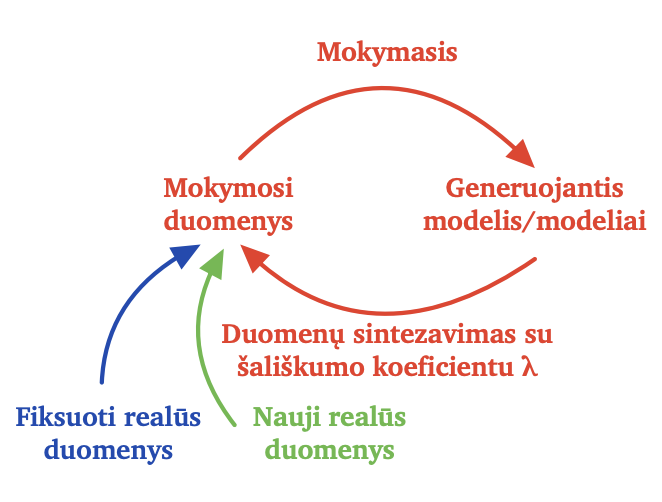
\includegraphics[scale=0.7]{img/valgantysCiklai.png}
    \caption{
        \textbf{\cite{ModelsGoMAD} straipsnyje pavaizduoto save valgančių ciklų vaizdo atvaizdavimas lietuvių kalba.} Paveiksle galima matyti tris skirtingus save valgančius ciklus:
    }
    \label{img:ciklai}
    
    \begin{itemize}
        \item \textbf{\textcolor{raudona}{Pilnai sintetinių duomenų ciklą}}: apibūdina ciklą, kuriame naudojami tik pilnai sintetiniai duomenys.
        \item \textbf{Sintetinių duomenų augmentacijų ciklą}: šiame cikle naudojami \textbf{\textcolor{melyna}{fiksuoti realūs duomenys}} kartu su \textbf{\textcolor{raudona}{pilnai sintetiniais duomenimis}}.
        \item \textbf{Ciklą su šviežiais duomenimis}: ciklas, apima \textbf{\textcolor{zalia}{naujus realius duomenis}} kartu su \textbf{\textcolor{raudona}{pilnai sintetiniais duomenimis}}.
    \end{itemize}

    Paveikslo elementuose taip pat matomas šališkumo parametras \textbf{\textcolor{raudona}{\(\lambda\)}}, kuris nusako, kaip atrodys generuojamų pavyzdžių kokybės ir įvairovės pasiskirstymas. \textbf{\textcolor{raudona}{\( \lambda \)}} kontroliuoja, kiek modelis generuodamas naujus duomenis orientuojasi į dažniausiai pasitaikančias reikšmes (modą) ir kiek atsižvelgia į mažiau tikėtinas, tačiau įvairesnes reikšmes (įvairovę). Skirstinio kraštų paaiškinimas žr. \ref{img:uodegos} pav.

    \begin{itemize}
        \item Jei \textbf{\textcolor{raudona}{\(\lambda = 1 \)}} (nešališkas generavimas): modelis naudoja visą duomenų skirstinį, įskaitant ir retas reikšmes, kurios dažnai yra duomenų uodegose. Rezultatas: didelė įvairovė, tačiau kai kurios sugeneruotos reikšmės būna prastesnės kokybės, nes jos neatspindi pagrindinių skirstinio bruožų.
        \item Jei \textbf{\textcolor{raudona}{\(\lambda = 0 \)}} (visiškai šališkas generavimas): modelis daugiausia dėmesio skiria skirstinio centrui – dažniausiai pasitaikančioms reikšmėms (moda). Rezultatas: aukšta kokybė, tačiau sugeneruoti duomenys labai panašūs, prarandama įvairovė.
    \end{itemize}
\end{figure}




Taip pat svarbu paminėti, kad ryškią rolę save valgančiuose cikluose turi ir duomenų atrankos šališkumo kiekvienoje mokymosi iteracijoje koeficientas \(\lambda \). Alemohammad et al. tyrime\cite{ModelsGoMAD} nurodo, jog visai netaikant šio koeficiento modeliai nustoja generuoti kokybiškus ir įvairius duomenis, kas ir yra DI modelų kolapso bruožas. Taikant \(\lambda\), situacija kinta - kokybė gali būti visai neblogai išlaikoma, bet duomenų įvairovė smarkiai sumažėja, kas taip pat yra kolapso bruožas. 

\subsubsubsection{Sintetinių duomenų ciklai}

Sintetinių duomenų ciklai (angl. \textsl{fully synthetic loop}), tai tokie save valgantys ciklai, kurie apima DI modelių mokymą tik su jų pačių sugeneruotais duomenimis. Šiuose cikluose visiškai pašalinami realūs duomenys, o modelis remiasi tik anksčiau sugeneruotais rezultatais. Strategija rinktis taip mokyti modelį  dažniausiai sukelia greitą DI modelių kolapsą, nes klaidos kaupiasi kiekvienoje naujoje modelio mokymosi kartoje, o taip smarkiai keičiasi sugeneruotų duomenų ir originalių duomenų skirstinio panašumai - t.y. jie tampa vis labiau nepanašūs.



\subsubsubsection{Sintetiniai augmentacijų ciklai}
Sintetiniai augmentacijų ciklai (angl. \textsl{synthetic augmentation loop}) naudoja realių ir DI modelio sugeneruotų (sintetinių) duomenų derinį. Modelis mokosi iš fiksuotos realių duomenų imties, papildytos sintetiniais duomenimis, siekiant padidinti duomenų kiekį. Nors šis metodas lėčiau veda prie DI modelių kolapso nei visiškai sintetiniai ciklai, vis tiek galų gale sugeneruotų duomenų kokybė ir įvairovė mažėja, nes fiksuota realių duomenų dalis negali visiškai kompensuoti klaidų kaupimosi per visas iteracijas.


\subsubsubsection{Ciklai su šviežiais duomenimis} \label{CiklaiSuSvieziaisDuomenimis}
Ciklai su šviežiais duomenimis (angl. \textsl{fresh data loop}) naudoja šviežių realių duomenų ir sintetinės informacijos derinį. Šiuose cikluose realių duomenų imtis nuolat atnaujinama, todėl modelis turi prieigą prie naujų realių (žmogaus kurtų) duomenų. Duomenų atnaujinimo ciklai su šviežiais duomenimis yra efektyviausi užkertant kelią DI modelių kolapsui, nes  pirminiai apmokyto modelio variantai bus galų gale pamiršti. Alemohammad et al. \cite{ModelsGoMAD} net pastebėjo, jog tokiu variantu, kai modelį mokome šviežiais duomenimis, sintetinių duomenų naudojimas gali net gi pagerinti modelio sugeneruotų duomenų kokybę ir įvairovę. Bet, jei naudojame per daug DI modelio sugeneruotų (sintetinių) duomenų kokybė gali kristi. 



\subsection{Kaip apsisaugoti nuo DI modelių kolapso?}

Nors modelių kolapso tema yra gana nauja (pirmieji straipsniai, kuriuose pateiktas šio reiškinio apibrėžimas, pasirodė tik 2024 metais \cite{AICollapseNature}), ji tampa vis svarbesnė. Dabar, kai vis daugiau DI sugeneruotų duomenų pasiekia internetą ir internete talpinami modeliai tampa mokymo duomenų šaltiniu, kyla grėsmė, kad kolapsas taps nevaldoma problema, todėl svarbu sukurti prevencines priemones, kurios užtikrintų ilgalaikį DI modelių stabilumą ir patikimumą.

\subsubsection{Siūlomi sprendiniai mažinti DI kolapso rizikas}

Dohmatob et al. \cite{DesniuPasiulymai} tyrime pateikia įvairius praktinius sprendimus, skirti apsaugoti DI modelius nuo kolapso. Pateikiami sprendiniai:

\begin{enumerate}
    \item \textbf{Realių ir DI sugeneruotų duomenų maišymas}:
    \\
        Straipsnyje siūloma reguliariai įtraukti nedidelį kiekį naujų realių duomenų į mokymo rinkinius. Tokį pastebėjimą, kad tinkamas duomenų atrinkimas gali net pagerinti modelio našumą aprašyta ir \ref{CiklaiSuSvieziaisDuomenimis} skyrelyje (informacija iš \cite{ModelsGoMAD} straipsnio). Tai padeda išlaikyti duomenų įvairovę ir stabilumą, neleidžiant mokymo rinkiniams per daug nukrypti nuo pradinio duomenų skirstinio. Šis metodas puikiai išspręstų problemas, susijusias su retų duomenų praradimu ir skirstinių skirtumais, kurie aptarti \ref{KodelKolapsas} ( \cite{AICollapseNature} straipsnio aptarime). Straipsnyje \cite{DesniuPasiulymai} taip pat pabrėžiama, kad glaima modeliuose bandyti atrasti geriausią naujų realių duomenų ir DI modelio sugeneruotų duomenų santykį darant empyrinius bandymus.
     
        Straipsnyje \cite{DesniuPasiulymai}
        aptariama, kaip tinkamas realių ir sugeneruotų duomenų santykis gali padėti stabilizuoti modelių mokymą ir net pagerinti jų našumą (žr. \ref{img:gorkking} pav.). Tyrimo metu empiriškai analizuojamos skirtingos naujų realių duomenų ir sintetinių duomenų proporcijos. Pastebėta, kad skirtingiems modeliams galima atrasti tam tikrą slenkstinę vertę, kur modelis veiks geriausiai. 


        \begin{figure}[H]
    \centering
    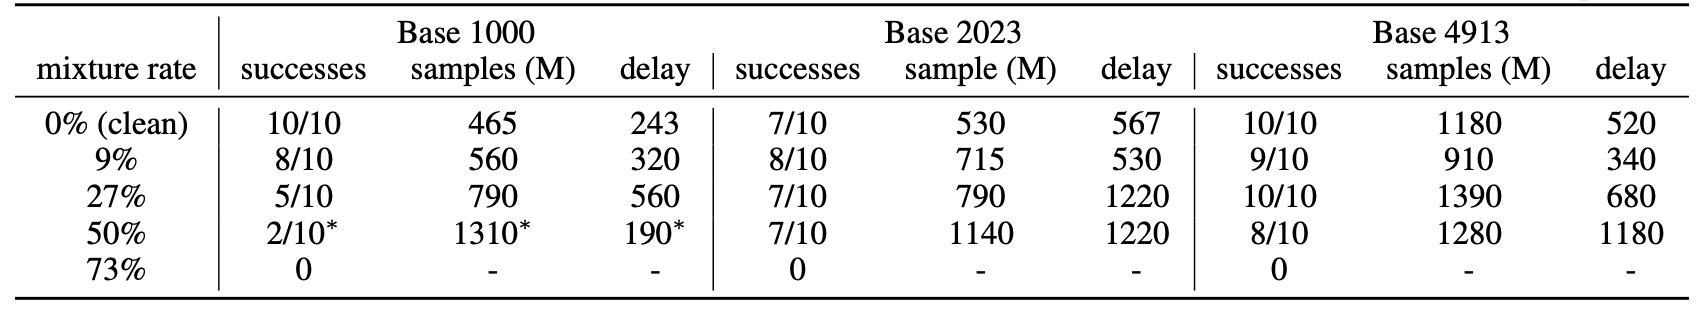
\includegraphics[scale=0.5]{img/gorkking.png}
    \caption{
        \textbf{\cite{DesniuPasiulymai} straipsnyje pateikta lentelė iliustruojanti šviežių realių duomenų ir modelio sukurtų duomenų santykio pasiskirstymo efektą DI modelių kolapsui.} 
        Procentai lentelėje rodo priemaišų procentą (angl. \textsl{mixture rate}) ir modelių sugebėjimą išmokti rasti didžiausią bendrą daliklį (angl. \textsl{GCD - greatest common divisor}).
        }
       \label{img:gorkking}
        \textbf{Sintetinių duomenų procentas (angl. \textsl{mixture rate})} nurodo, kiek realių duomenų maišoma su sintetiniais (0\% reiškia, kad naudojami tik švarūs duomenys). \textbf{Skaičių sistemos bazė (angl. \textsl{Base}) (pvz., 1000, 2023, 4913)} nurodo, kokia skaičių sistema užkoduoti duomenys, pagal kuriuos ieškomas didžiausias bendras rodiklis (bazė = 2 reiškia dvejetainę sistemą su elementais $A=\{00,01,10,11\}$). \textbf{Duomenų skaičius (angl. \textsl{Samples (M)})} yra nurodomas milijonais. \textbf{Modelių kiekis, kurie sėkmingai grąžino teisingus duomenis (angl. \textsl{Successes})}, rodo, kiek modelių iš 10 galimų sugebėjo išmokti užduotį (8/10 reiškia, kad 8 iš 10 modelių pasiekė sėkmę). Galiausiai, \textbf{vėlavimas (angl. \textsl{delay})} nurodo laikotarpį (mėginiais), reikalingą grokking fenomenui pasireikšti, kai modelis pereina nuo stagnacijos prie sėkmingo mokymosi; didesnis skaičius rodo ilgesnį laikotarpį iki efektyvaus mokymosi.
        
        Lentelė rodo, kad 27\% sintetinių duomenų yra geriausias šiam modeliui, nes modelis greičiau pasiekia grokking ir taip pat sugeba beveik visi modeliai pasiekti tikslą.

        
        Lentelė aiškiai iliustruoja grokking fenomeną ir atskleidžia, kaip tinkamas realių ir sintetinių duomenų santykis gali lemti modelio našumą.

        Gorkking fenomenas nutinka, kai nneuroniniai tinklai tam tikrose mokymosi užduotyse pradeda generalizuoti gerokai vėliau, nei įvyksta jų persimokymas \cite{grokking}.
    %}
    %\label{img:gorkking}
\end{figure}



    \item \textbf{Tikslinis duomenų kuravimas}:
    
        Rekomenduojama papildyti mokymo rinkinius trūkstamais \enquote{uodegos} duomenimis – tai yra retais ir įvairiais pavyzdžiais, kurie dažnai neįtraukiami į įprastus duomenų rinkinius.
        Toks požiūris sumažina ankstyvojo kolapso riziką minėtą 1.1 skyrelyje, nes modeliai išmoksta geriau reprezentuoti įvairius duomenų pasiskirstymo elementus. Kaip paaiškinta skyriuje poskyryje 1.2.1.2., uodegų nykimas kaip viena iš DI modelių kolapso priežasčių.
   

    \item \textbf{Reguliarūs kokybės tikrinimai}:
    
        Straipsnyje siūloma įdiegti mechanizmus, leidžiančius nuolat stebėti sugeneruotų duomenų kokybę ir įvairovę. Tai padėtų laiku aptikti DI modelių kolapso požymius ir koreguoti mokymo procesą prieš modeliui visai sugriųvant.
    

    \item \textbf{Teisinis reguliavimas ir skaidrumas}:
    
         Rekomenduojama privalomai ženklinti DI modelių sugeneruotus duomenis žyma (angl. \testsl{watermark}), kad jie būtų lengvai atskiriami nuo realių duomenų. Taip pat siūloma teisiškai reikalauti, kad DI sugeneruotas turinys būtų aiškiai pažymėtas viešuose duomenų rinkiniuose (internete), siekiant užtikrinti skaidrumą ir duomenų rinkinių kokybę. Toks pasiūlymas pateiktas ir \cite{ModelsGoMAD} straipsnyje. 
    
\end{enumerate}


\subsubsection{Europos sąjungos pastangos mažinti DI modelių kolapsą DI reglamente}

Europos Parlamento ir Tarybos priimtas reglamentas (DI aktas), kuris įsigalios 2026 rugpjūčio 2 dieną \cite{AIEuropeanAct}, siekia užtikrinti patikimą dirbtinio intelekto naudojimą visoje Europos Sąjungoje. Nors reglamente tiesiogiai neminima DI modelių kolapso problema, jame pateikiami straipsniai gali netiesiogiai prisidėti prie šio reiškinio rizikų mažinimo. 

\subsubsubsection{Duomenų žymėjimas}
Reglamento 2 skyriaus 10 straipsnio 2 punkto (c) dalyje reikalaujama tvarkyti ir žymėti duomenis. Šis žingsnis yra itin reikšmingas užkertant kelią DI modelių kolapsui, nes:

\begin{itemize}
    \item Aiškus realių ir sintetinių duomenų atskyrimas padeda išlaikyti šviežius duomenis.
    \item Tai sumažina galimybę užteršti mokymosi rinkinius DI modelių sugeneruotais duomenimis (sintetiniais duomenimis), kas yra pagrindinė kolapso priežastis aptarta \cite{ModelsGoMAD}.
\end{itemize}

\subsubsubsection{Šališkumo tikrinimas}
To paties straipsnio (f) punktas pabrėžia būtinybę reguliariai tikrinti duomenų šališkumą, ypač jei šie duomenys daro įtaką ateities mokymo kartoms. Šališkumo tikrinimas padėtų sumažinti:

\begin{itemize}
    \item  Klaidingų duomenų kaupimo riziką - skirstinių uodegų sunykimo.
\end{itemize}

\subsubsubsection{Sintetinės medžiagos žymėjimas}
Reglamento 4 skyriaus 2 punkte numatyta, kad bendrosios paskirties DI sistemos, kurios generuoja medžiagą naudotojui, turi pažymėti šią medžiagą kaip sugeneruotą DI (kaip sintetinius duomenis). Ši priemonė padeda:

\begin{itemize}
    \item Atpažinti sintetinius duomenis, sumažinant jų nekontroliuojamo įtraukimo į realius duomenų rinkinius riziką.
    \item Mažinti modelio degradacijos galimybes. Kaip aptarta \cite{AICollapseNature} ir \cite{DesniuPasiulymai}, per didelis sintetinių duomenų kiekis sukelia skirstinių poslinkio ir retų duomenų praradimo klaidas.
\end{itemize}

Svarbu paminėti, jog duomenų žymėjimas ir šališkumo tikrinimas apsaugoja tik didelės rizikos DI sistemas, nes reglamente šie punktai taikomi tik šiom sistemoms. Didelės rizikos DI sistemos yra tokios, kurios kelia didelę riziką Europos sąjungos piliečių sveikatai, saugumui ar pagrindinėms teisėms, tačiau kurių svarbi socialinė ir ekonominė nauda atsveria šias rizikas.

Apibendrinant, duomenų žymėjimas ir šališkumo kontrolė tiesiogiai sprendžia duomenų kokybės ir įvairovės klausimus, kurie yra esminiai norint apsaugoti modelius nuo DI kolapso. Sintetinių duomenų atpažinimas padeda efektyviai valdyti švarius ir užtikrina, kad DI sistemų sugeneruota informacija būtų naudojama atsakingai.




\section{Eksperimentas}
\subsection{Eksperimento metodai}
Eksperimento tikslas identifikuoti ciklų, kuriuose modeliai mokymuisi naudoja sintetinius duomenis, vizualius pokyčius nuotraukose. Šiuo eksperimentu siekta palyginti keturių skirtingų ciklų efektyvumą, pasitelkiant variacinio autoenkoderio (angl. \textsl{Variational Autoencoder} (VAE)) gilųjį neuroninį tinklą ir MNIST \cite{MNIST} duomenų rinkinį. Lyginami šie straipnyje \cite{ModelsGoMAD} išskirti ciklai:
\begin{enumerate}
    \item Tik sintetinių duomenų ciklai.
    \item Sintetinių duomenų ciklai su augmentacijomis.
    \item Ciklai su šviežiais duomenimis.
    \item Standartinio modelio mokymas nepriklausantis save valgantiems ciklams.
\end{enumerate}

\subsubsection{Naudoti įrankiai ir metodai}

\begin{itemize}
    \item \textbf{Programavimo aplinka:} Google Colab/ Visual Studio Code;
    \item \textbf{Programavimo kalba:} Python;
    \item \textbf{Modelio architektūra:} variacinis automatinis koduotojas (VAE), paremtas \cite{DeepLearningPython} knygoje pasiūlyta architektūra;
    \item \textbf{Duomenų rinkinys:} MNIST.
\end{itemize}


MNIST rinkinys buvo pasirinktas dėl jo plačiai paplitusio naudojimo kaip pavyzdinio duomenų rinkinio DI modelių mokymui, taip pat dėl to, kad jis buvo naudojamas kolapsui atvaizduoti tyrime \cite{ModelsGoMAD}. Minėtame tyrime buvo nagrinėjamas sintetiniais duomenimis pagrįstų ciklų poveikis DI modeliams keičiant parametrą \(\lambda\) (lambda efektų paaiškinimas žr. \ref{img:ciklai} pav.). Visgi, šiame eksperimente pasirinkta nagrinėti ir kitų ciklų vizualius pokyčius, nekeičiant parametro \(\lambda\). 

VAE tinklas buvo pasirinktas atsižvelgiant į \cite{AICollapseNature} tyrimą, kur šiame modelyje pasireiškė specifinės klaidos, susijusios su modelių kolapsu (klaidos aptartos 1.2.1.1. skyriuje). Eksperimentu siekta patikrinti, ar šios klaidos ne tik aprašomos literatūroje, bet ir gali būti vizualiai pastebimos kitokiuose duomenų rinkiniuose, nei žmonių nuotraukos. Be to, minėtuose tyrimuose buvo naudoti kiti metodai, \cite{ModelsGoMAD} straipsnyje duomenys apdoroti naudojant DDPM modelį su MNIST duomenų rinkiniu, o \cite{AICollapseNature} išviso nepateikė informacijos apie naudotą duomenų rinkinį.

\subsubsection{Eksperimentinė aplinka}

Visiems modeliams mokyti buvo naudojamos 5 generacijos. Vieną generaciją sudarė 20 epochų, o duomenų rinkinio dydis (angl. \textsl{batch size}) buvo 256. Pasirinkimas vykdyti 20 epochų su 256 rinkinio dydžiu per vieną generaciją paremtas \cite{ModelsGoMAD} tyrimo eksperimentų metodologija. Pasirinkimas vykdyti 5 generacijas priimtas, nes tyrime \cite{AICollapseNature} pastebėta, kad modelio kolapsas naudojant VAE gali būti pastebimas jau ankstyvosiose generacijose.

Po kiekvienos mokymosi generacijos modelį mokome iš naujo renmdamiesi \cite{ModelsGoMAD} metodu. Tam, kad modeliai kažkiek išmoktų užduotį pirmos generacijos metu modelis mokosi su MNIST orginaliais duomenimis. 
% Realių duomenų procentas epochoje (nuo antros generacijos) nustatytas 75\% vykdant sintetinių augmentacijų ciklą, o vykdant ciklą su šviežiais duomenimis realių naujų duomenų buvo taip pat naudota 75\%.


\begin{itemize}
    \item \textbf{Sintetinių duomenų ciklas} -
    Duomenų rinkinio dydis: 256 
    \item \textbf{Sintetinių augmentacijų ciklas} -
    Duomenų rinkinio dydis: 256, realių duomenų procentas epochoje (nuo antros generacijos): 75\%
    \item \textbf{Ciklas su šviežiais duomenimis} -
    Duomenų rinkinio dydis: 256, realių šviežių duomenų procentas epochoje (nuo antros generacijos): 75\%
    \item \textbf{Standartinio modelio mokymas nepriklausantis save valgantiems ciklams} -
    Duomenų rinkinio dydis: 256
\end{itemize}

Po kiekvienos mokymosi generacijos modelis yra mokomas iš naujo, remiantis \cite{ModelsGoMAD} metodu. Siekiant, kad modeliai bent iš dalies išmoktų užduotį, pirmosios generacijos metu modelis yra mokomas naudojant MNIST originalius duomenis. 

% Pradedant nuo antrosios generacijos, sintetinių duomenų procentas epochoje nustatytas 25\% tiek vykdant sintetinių augmentacijų ciklą, tiek vykdant ciklą su šviežiais duomenimis.



Pasirinkimas naudoti nedidelį gilųjį neuroninį tinklą, mažą duomenų rinkinį ir apribotą epochų bei generacijų skaičių priimtas, nes tai leidžia sumažinti energijos sąnaudas, prisidedant prie tvaresnio mokslinio darbo, kaip pabrėžia \cite{energy_2019}. 




\subsection{Eksperimento rezultatai}

\subsubsection{Sintetinių duomenų ciklas}
VAE modelio kolapsas, naudojant tik sintetinius duomenis, buvo labai ryškus (žr. \ref{img:sintetiniai_gen_1_5} pav.). Kaip ir tikėtasi, duomenys smarkiai suvienodėjo – iš rinkinio netgi dingo kai kurie skaitmenys. Atpažįstami tik pusę skaitmenų (0, 3, 6, 8, 9), tačiau dauguma jų yra labai blankūs. Tuo tarpu pirmoje generacijoje matomi visi skaičiai nuo 1 iki 9, kaip ir tikėtina naudojant MNIST duomenų rinkinį (žr. \ref{img:sintetiniai_gen_1_5} pav.).

\begin{figure}[H]
    \centering
    % First image
    \begin{subfigure}[t]{0.45\textwidth} % Adjust width as needed
        \centering
        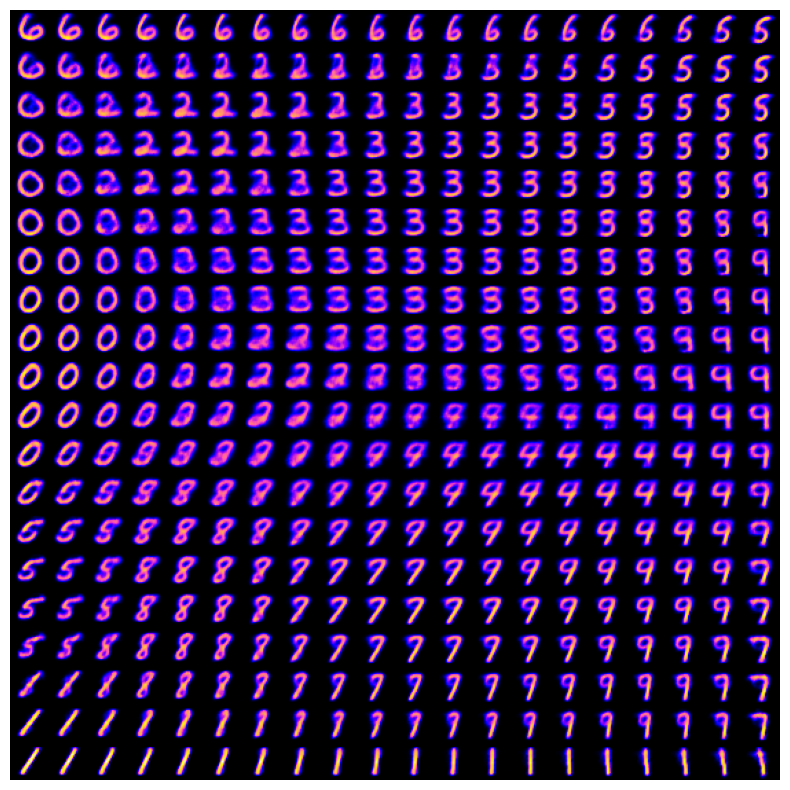
\includegraphics[scale=0.40]{img/synthetic_generation_1.png}
        \caption{Pirma genereracija.}
        \label{img:image1}
    \end{subfigure}
    \hfill % Adds some horizontal space
    % Second image
    \begin{subfigure}[t]{0.45\textwidth} % Adjust width as needed
        \centering
        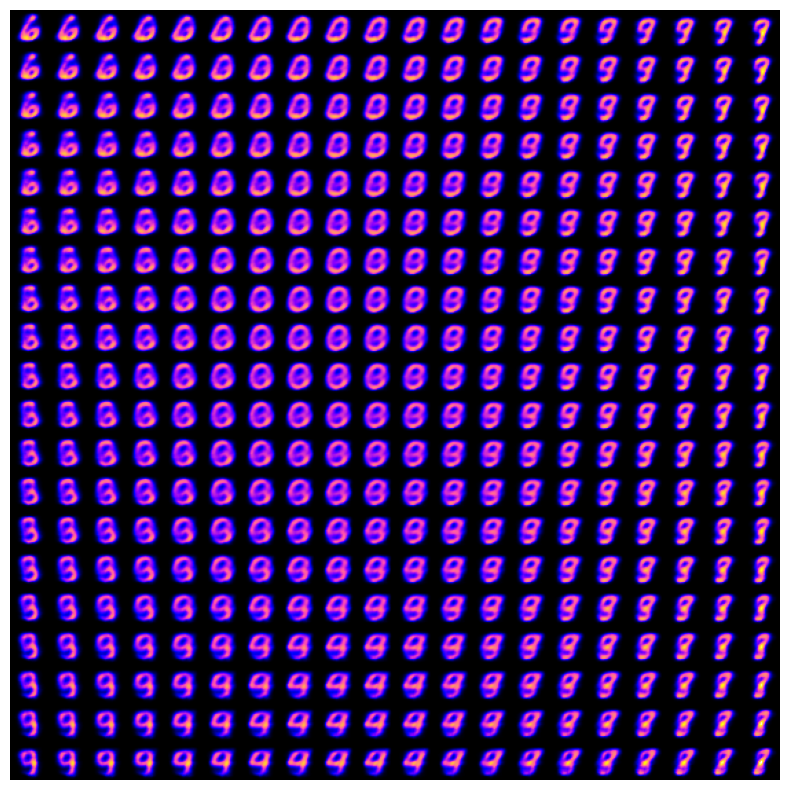
\includegraphics[scale=0.40]{img/synthetic_generation_2.png}
        \caption{Penkta generacija.}
        \label{img:image2}
    \end{subfigure}
    \caption{\textbf{Pirmosios ir penktosios sintetinių duomenų ciklo generacijos palyginimas}.Matyti, kad po penktosios mokymosi generacijos tinklo išvesti duomenys smarkiai suvienodėjo, o pirmoje generacijoje modelis dar gana tiksliai vaizdavo visus skaičius nuo 0 iki 9.}
    \label{img:sintetiniai_gen_1_5}
\end{figure}

\subsubsection{Sintetinių augmentacijų ciklas}
Išvestys po pirmos ir penktos generacijos smarkiai nepakito (žr. \ref{img:augmentation_gen_1_5} pav.).

\begin{figure}[H]
    \centering
    % First image
    \begin{subfigure}[t]{0.45\textwidth} % Adjust width as needed
        \centering
        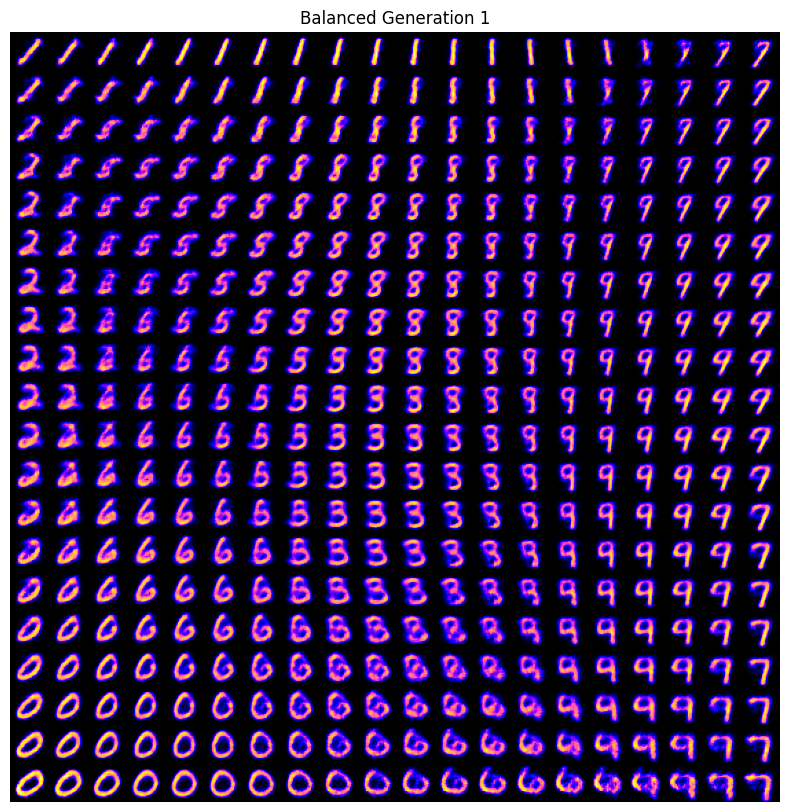
\includegraphics[scale=0.40]{img/real_synthetic_generation_1.png}
        \caption{Pirma genereracija.}
        \label{img:image1}
    \end{subfigure}
    \hfill % Adds some horizontal space
    % Second image
    \begin{subfigure}[t]{0.45\textwidth} % Adjust width as needed
        \centering
        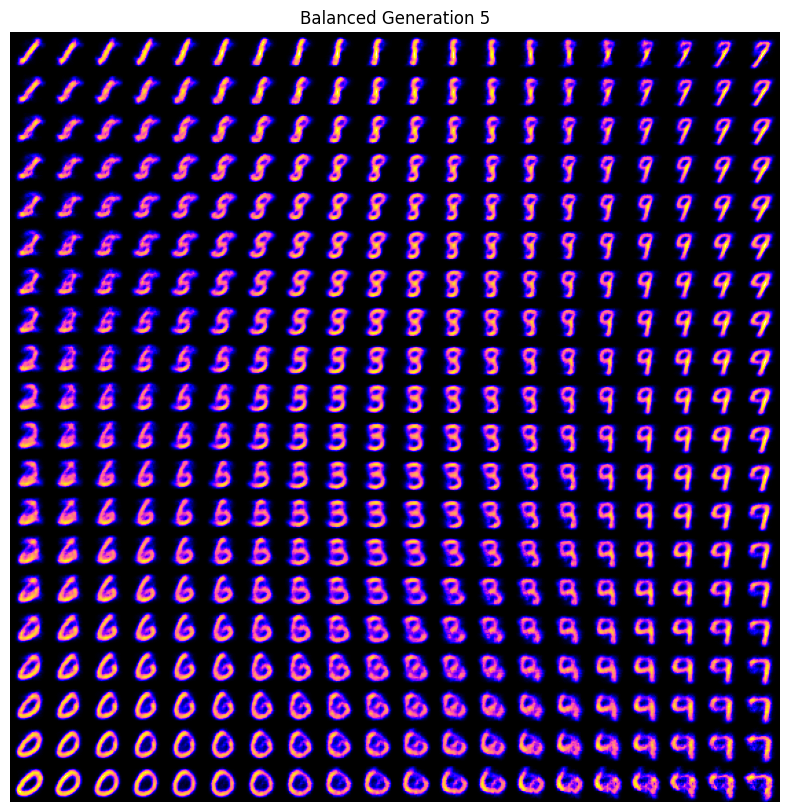
\includegraphics[scale=0.40]{img/real_synthetic_generation_5.png}
        \caption{Penkta generacija.}
        \label{img:image2}
    \end{subfigure}
    \caption{\textbf{Pirmosios ir penktosios sintetinių augmentacijų ciklo generacijos palyginimas}.Matyti, kad tinklo išvesti duomenys po pirmosios ir penktosios mokymosi generacijų smarkiai nepasikeitė, tačiau tapo šiek tiek sulieti penktoje generacijoje.}
\label{img:augmentation_gen_1_5}
\end{figure}





\subsubsection{Ciklas su šviežiais duomenimis}
Išvestys smarkiai nepakito, gal kiek ryškesni pasidarė (žr. \ref{img:fresh_gen_1_5} pav.).
\begin{figure}[H]
    \centering
    % First image
    \begin{subfigure}[t]{0.4\textwidth} % Adjust width as needed
        \centering
        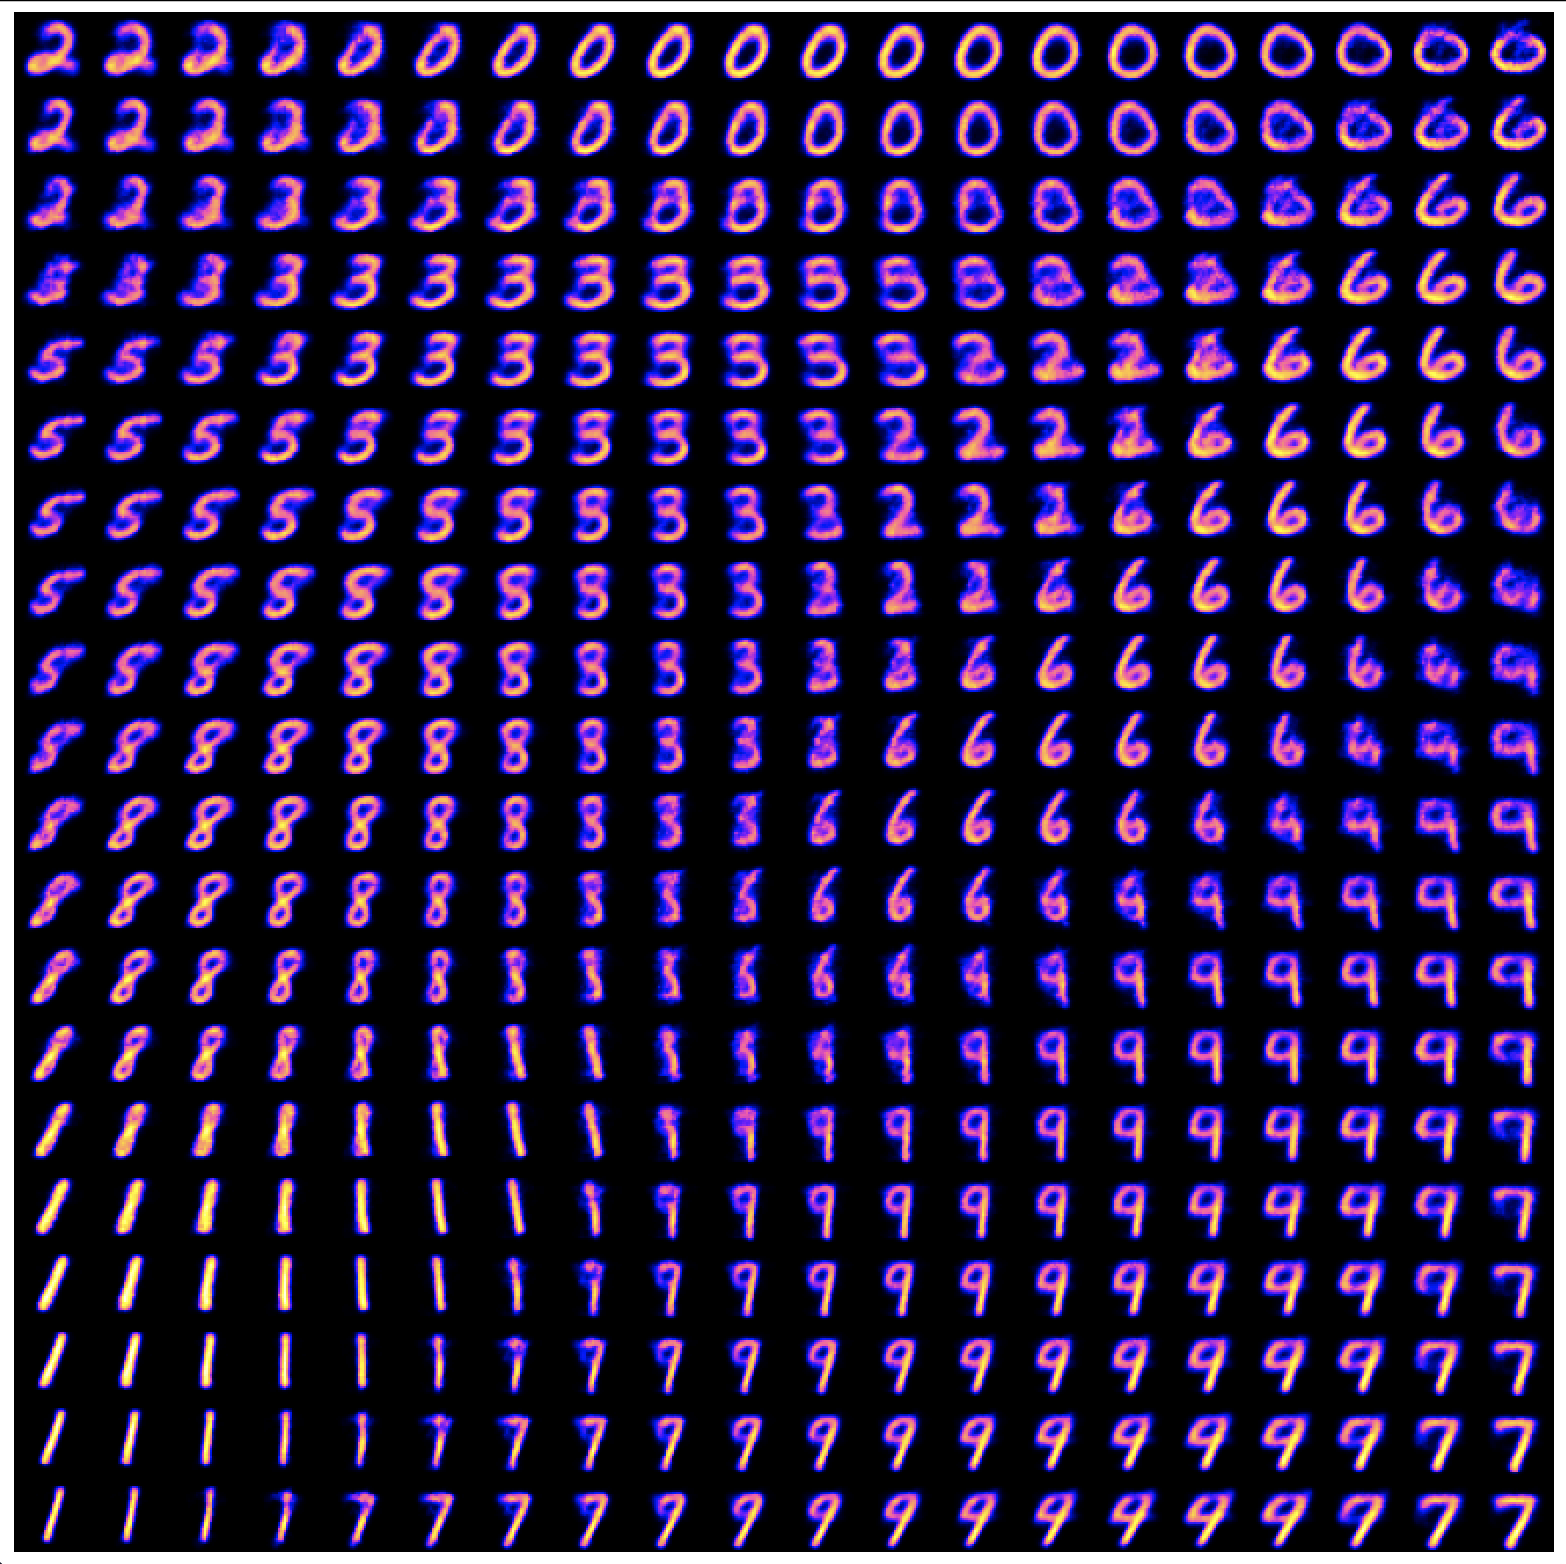
\includegraphics[scale=0.28]{img/fresh_generation_1.png}
        \caption{Pirma genereracija.}
        \label{img:image1}
    \end{subfigure}
    \hfill % Adds some horizontal space
    % Second image
    \begin{subfigure}[t]{0.45\textwidth} % Adjust width as needed
        \centering
        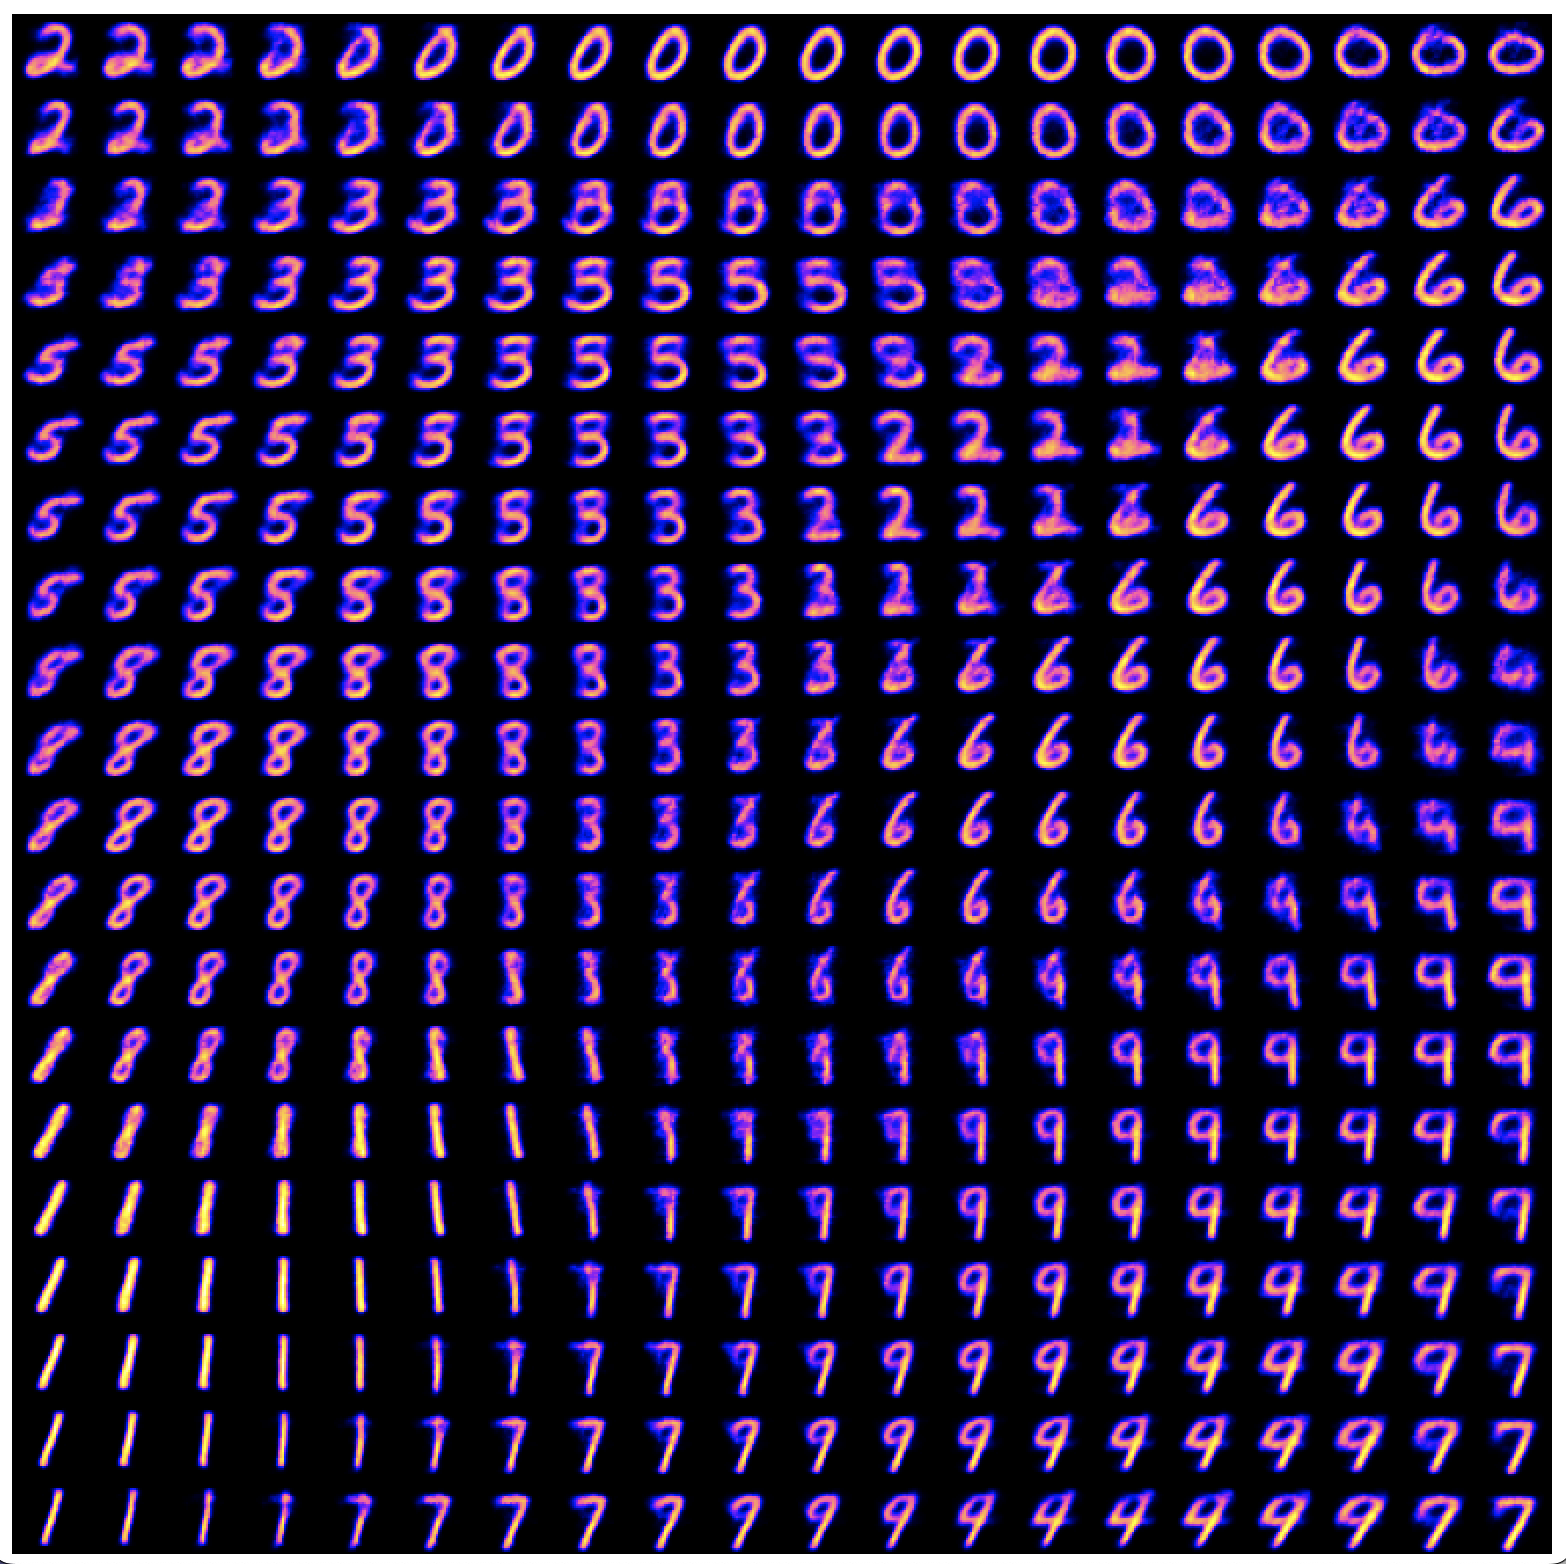
\includegraphics[scale=0.28]{img/fresh_generation_5.png}
        \caption{Penkta generacija.}
        \label{img:image2}
    \end{subfigure}
    \caption{\textbf{Pirmosios ir penktosios ciklo su šviežiais duomenimis generacijos palyginimas.}.Matyti, kad tinklo išvesti duomenys po pirmosios ir penktosios mokymosi generacijų smarkiai nesiskiria.}
    \label{img:fresh_gen_1_5}
\end{figure}


\subsubsection{Standartinio modelio mokymas nepriklausantis save valgantiems ciklams}

Atliktas eksperimentas parodė, kad modelis turi gebėjimą mokytis, vizualūs pokyčiai tarp generacijų atskleidžia skaičių paryškėjimą (žr. \ref{img:original_gen_1_5} pav.).

\begin{figure}[H]
    \centering
    % First image
    \begin{subfigure}[t]{0.45\textwidth} % Adjust width as needed
        \centering
        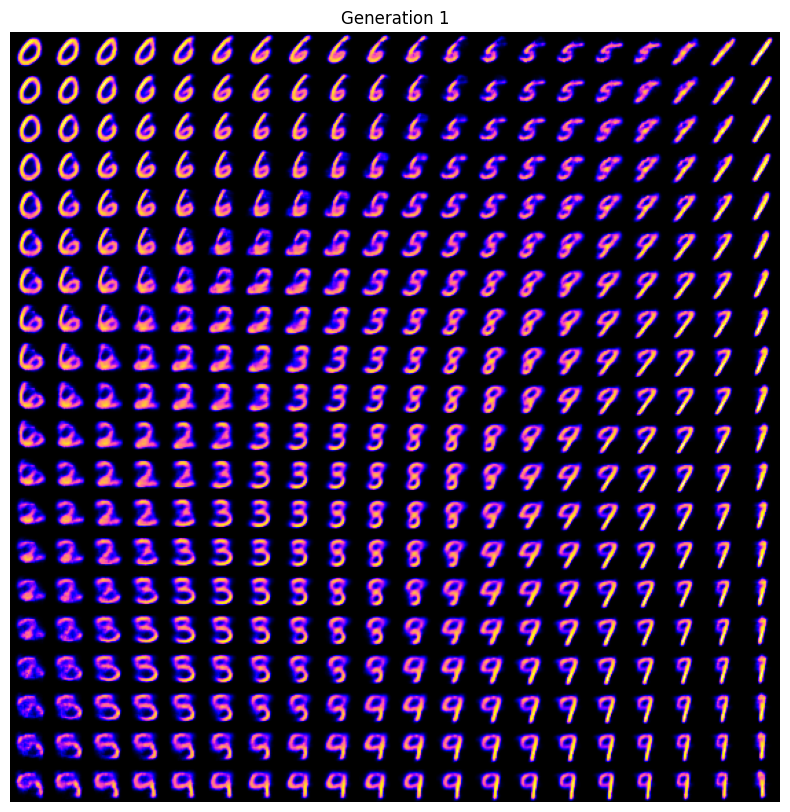
\includegraphics[scale=0.40]{img/original_generation_1.png}
        \caption{Pirma genereracija.}
        \label{img:image1}
    \end{subfigure}
    \hfill % Adds some horizontal space
    % Second image
    \begin{subfigure}[t]{0.45\textwidth} % Adjust width as needed
        \centering
        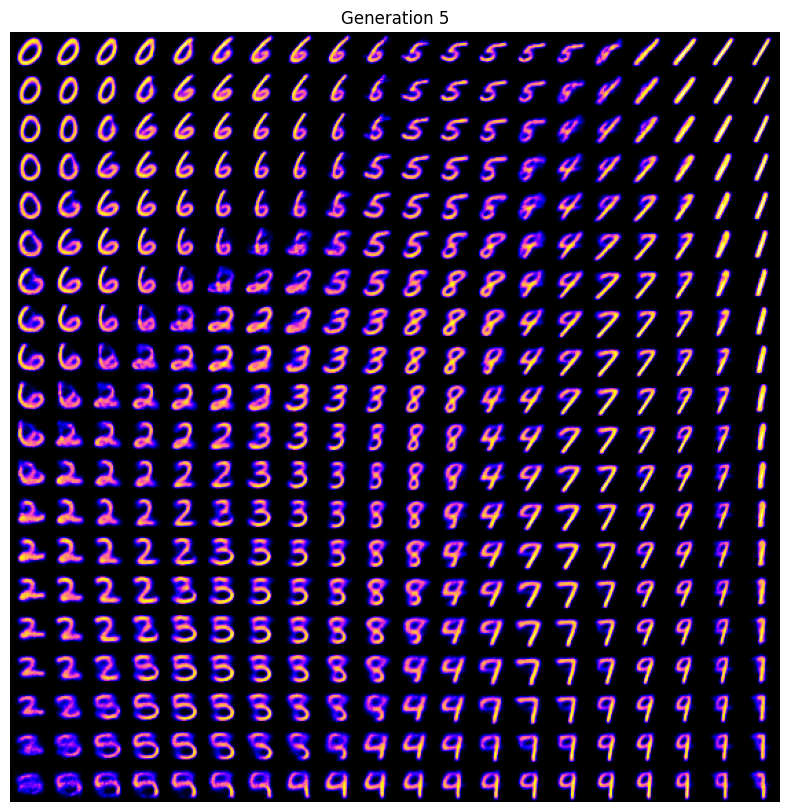
\includegraphics[scale=0.40]{img/original_generation_5.png}
        \caption{Penkta generacija.}
        \label{img:image2}
    \end{subfigure}
    \caption{\textbf{Pirmosios ir penktosios generacijų su standartiniu apmokymu palyginimas}.Matyti, kad tinklo išvesti duomenys po pirmosios ir penktosios mokymosi generacijų pakito į gerąją pusę, tačiau didelių skirtumų nėra.}
    \label{img:original_gen_1_5}
\end{figure}


\subsection{Rezultatų aptarimas}

Rezultatai patvirtina, kad kolapsas yra akivaizdus net ir naudojant kitus duomenų rinkinius, tokius kaip MNIST, sintetinių duomenų cikle. Naudojant tik sintetinius duomenis, kolapso požymiai pasireiškia jau po nedidelio generacijų skaičiaus (5): kai kurie skaičiai tampa sunkiai atpažįstami, o skaičių įvairovė išnyksta. 

Tačiau taikant kitas duomenų maišymo strategijas, tokias kaip realių ir sintetinių duomenų maišymas arba naujų realių ir sintetinių duomenų kombinavimas, negalime teigti, kad VAE neuroninio tinklo kolapsas įvyko ar kad modelis pradėjo veikti geriau. Tikėtina, kad maišius realius ir sintetinius duomenis kolapso rizika galėjo būti atidėta į tolesnes generacijas (\cite{AICollapseNature}). Be to, naudojant naujų realių duomenų maišymą, galimai nebuvo pasirinktas optimalus santykis, nes trūko resursų empyriniam tyrimui atlikti (tyrimas yra siūlomas \cite{DesniuPasiulymai} straipsnyje).



\section{Rezultatai ir išvados}

\subsection{Rezultatai}
Atlikus eksperimentą aprašytą skyriuje 2. buvo pasiekti tokie rezultatai:
\begin{itemize}
    \item \textbf{Sintetinių duomenų ciklas:}
    \begin{itemize}
        \item Po penktosios generacijos VAE modelis parodė stiprų kolapso efektą: prarastos daugelio skaitmenų įvairovės savybės.
        \item Tik keli skaitmenys (0, 3, 6, 8, 9) buvo atpažįstami, tačiau ir jie buvo labai blankūs.
    \end{itemize}
    \item \textbf{Sintetinių augmentacijų ciklas:}
    \begin{itemize}
        \item Vizualiai rezultatų kokybė nuo pirmos iki penktos generacijos žymiai nesiskyrė.
        \item Pastebėtas nežymus vaizdų suliejimas.
    \end{itemize}
    \item \textbf{Ciklas su šviežiais duomenimis:}
    \begin{itemize}
        \item Po penktos generacijos tinklo išvestys tapo šiek tiek ryškesnės.
        \item Įvairovės praradimas nebuvo pastebėtas.
    \end{itemize}
    \item \textbf{Standartinio modelio mokymas:}
    \begin{itemize}
        \item Po penktos generacijos duomenų kokybė pagerėjo, vaizdai tapo ryškesni ir aiškesni.
        \item Modelis parodė gebėjimą mokytis.
    \end{itemize}
\end{itemize}

\subsection{Išvados}
Pagal literatūros apžvalgą ir atliktą eksperimentą padarytos tokios išvados:
% DI modelių kolapsas yra procesas, kylantis dėl modelių mokymo su jų pačių sugeneruotais duomenimis. Šis reiškinys lemia informacijos ir duomenų skirstinio struktūros praradimą, kuris daro neigiamą poveikį modelių veikimui ir patikimumui. Naujų realių duomenų įtraukimas į mokymo procesą bei jų žymėjimo užtikrinimas yra esminiai veiksniai, padedantys sumažinti kolapso riziką. Kadangi DI modelių kolapsas gali turėti reikšmingų ekonominių, ekologinių ir socialinių pasekmių, būtina skirti ypatingą dėmesį šios problemos valdymui.

% Vienas iš būdų išvengti DI modelių kolapso yra tinkamas šališkumo kontrolės parametro \(\lambda\) nustatymas. Šis parametras padeda išlaikyti pusiausvyrą tarp sugeneruotų duomenų kokybės ir įvairovės, tačiau jo taikymas reikalauja daugiau tyrimų siekiant suprasti poveikį skirtinguose modeliuose.

% Europos Sąjungos DI reglamentas taip pat prisideda prie kolapso rizikos mažinimo. Jame numatytos priemonės, tokios kaip duomenų žymėjimas ir šališkumo kontrolė, gali padėti užtikrinti didesnį modelių stabilumą. Tačiau reglamentas šiuo metu koncentruojasi tik į didelės rizikos DI sistemas ir įsigalios tik 2026 metų rugpjūčio 2 d. Dėl to kyla klausimų, kaip dabartiniai ir ateities DI modeliai, apdorojantys didelius informacijos srautus iš interneto iki 2026 metų bus paveikti DI modelių kolapso. Ateityje didelę vertę galėtų turėti duomenų bazės, kurios užtikrina tikrų duomenų saugojimą ir prieinamumą, nes DI modelių generuojami duomenys gali smarkiai užteršti DI modelių mokymosi duomenis.

% Pastebima, kad DI kolapso tema dar nėra pakankamai ištirta. Ypač trūksta tyrimų, kurie nagrinėtų sugeneruotų duomenų maišymo poveikį tarp skirtingų modelių, vykdančių panašias užduotis. Toks tyrimas galėtų geriau atspindėti dabartinę interneto duomenų struktūrą. 

\begin{itemize}
    \item \textbf{DI modelių kolapso pobūdis:}
    \begin{itemize}
        \item DI modelių kolapsas atsiranda, kai modeliai mokomi naudojant jų pačių sugeneruotus duomenis, o tai lemia duomenų įvairovės praradimą.
        \item Eksperimentai patvirtino, kad kolapsas sintetinių duomenų cikluose yra neišvengiamas ir pasireiškia jau po kelių generacijų.
    \end{itemize}
    \item \textbf{Maišymo strategijos efektyvumas:}
    \begin{itemize}
        \item Realūs ir sintetiniai duomenys (augmentacijos ir šviežių duomenų cikluose) sumažina kolapso riziką, tačiau netinkamas santykis šviežių duomenų cikluose gali sukelti kokybės praradimus, o sintetinių augmentacijų cikluose tik nutolinti Di modelių kolapsą.
        \item Naujų realių duomenų įtraukimas į mokymo procesą išlieka efektyviausiu būdu mažinti kolapso riziką.
    \end{itemize}
    \item \textbf{Reguliavimo svarba:}
    \begin{itemize}
        \item Europos Sąjungos DI reglamentas, apimantis duomenų žymėjimą ir šališkumo kontrolę, gali netiesiogiai padėti DI modeliams išvengti kolapso.
        \item Reglamentas įsigalios tik 2026 metais, todėl kolapso prevencijai būtina plėtoti alternatyvius sprendimus iki to laiko.
    \end{itemize}
\end{itemize}



\subsection{Rekomendacijos}

Atsižvelgiant į gautas išvadas, pateikiamos šios rekomendacijos:
\begin{itemize}
    \item \textbf{Mokslininkams:} Rekomenduojama tęsti tyrimus, siekiant geriau suprasti sintetinių ir šviežių realių duomenų santykio poveikį DI modelių stabilumui bei jų kokybei. Taip pat būtina gilintis į šališkumo kontrolės parametro \(\lambda\) reikšmę skirtingose generatyvinėse architektūrose ir mokymosi cikluose. Siūloma tyrinėti ilgalaikį sugeneruotų duomenų maišymo poveikį tarp skirtingų modelių ir jų rezultatų kokybę. Tai padėtų geriau suprasti dabartines ir būsimas interneto duomenų būsenas bei jų įtaką DI modelių stabilumui.
    \item \textbf{Praktikams:} Mokymo procesams svarbu užtikrinti, kad duomenų rinkiniai būtų reguliariai atnaujinami šviežiais realiais duomenimis, taip išlaikant įvairovę ir užkertant kelią modelių kolapsui. Reikėtų užtikrinti, kad sintetiniai duomenys būtų naudojami subalansuotai, neviršijant saugių proporcijų.
    \item \textbf{Politikos kūrėjams ir vykdytojams:} Siūloma Europos Sąjungos DI reglamente toliau stiprinti reikalavimus sugeneruotų duomenų žymėjimui ir kontrolės mechanizmams. Be to, reikėtų svarstyti įtraukti daugiau nuostatų, skirtų mažesnės rizikos DI sistemoms, kurios taip pat gali patirti kolapsą. Svarbu ir tai, kad ir kitos valdomieji kūnai kurtų kitus reglamentus ar įstatymus skirtus DI kolapso mažinimo tematikai. 
    \item \textbf{Bendruomenei:} Rekomenduojama didinti informuotumą apie DI modelių kolapso rizikas ir jų prevencijos svarbą. Švietimas šia tema gali padėti tiek naudotojams, tiek kūrėjams atsakingai naudoti DI technologijas. Taip pat svarbu atkreipti dėmesį į tai, kaip sistemų naudotojai prisideda prie duomenų kokybės, ir skatinti juos neteršti interneto modelių sugeneruotais duomenimis, kurie gali neigiamai paveikti būsimų modelių mokymosi procesus.

\end{itemize}


% Išvadose ir pasiūlymuose, nekartojant atskirų dalių apibendrinimų,
% suformuluojamos svarbiausios darbo išvados, rekomendacijos bei pasiūlymai.

\printbibliography[heading=bibintoc] % Literatūros šaltiniai aprašomi
% bibliografija.bib faile. Šaltinių sąraše nurodoma panaudota literatūra,
% kitokie šaltiniai. Abėcėlės tvarka išdėstoma tik darbe panaudotų (cituotų,
% perfrazuotų ar bent paminėtų) mokslo leidinių, kitokių publikacijų
% bibliografiniai aprašai (šiuo punktu pasirūpina LaTeX). Aprašai pateikiami
% netransliteruoti.

%\appendix  % Priedai
% Prieduose gali būti pateikiama pagalbinė, ypač darbo autoriaus savarankiškai
% parengta, medžiaga. Savarankiški priedai gali būti pateikiami kompiuterio
% diskelyje ar kompaktiniame diske. Priedai taip pat vadinami ir numeruojami.
% Tekstas su priedais siejamas nuorodomis (pvz.: \ref{img:mlp}).

%\section{Naudingi paveikslai ir grafikai}


\section{Eksperimente sukurti duomenys}
Duomenys talpinami \enquote{Google Drive} platformoje. Nuoroda: \url{https://drive.google.com/drive/folders/1cWRrLsbtK7NMCd0fewAJ3DNa9hOn2ZSj?usp=drive_link}

\appendix 
\end{document}


